\documentclass[12pt]{article}
\usepackage[utf8]{inputenc}
\usepackage[margin=1in]{geometry}
\usepackage{times}
\usepackage{multicol}
\usepackage{graphicx}
\usepackage{caption}
\usepackage{multirow}
\usepackage[table,xcdraw]{xcolor}

\newenvironment{Figure}
  {\par\medskip\noindent\minipage{\linewidth}}
  {\endminipage\par\medskip}

\raggedcolumns

% Please change the name if you can think of something better
\title{Support Vector Machines vs. Deep Learning on Speech Emotion Classification}
\author{
  Woloshyn, Christopher\\
  \texttt{cwolosh1@binghamton.edu}
  \and
  Lounsbury, Nathaniel\\
  \texttt{nlounsb1@binghamton.edu}
  \and
  Ma, Qiyang\\
  \texttt{qma1@binghamton.edu}
  }
\date{May 2020}


\begin{document}

\maketitle

\begin{abstract}
For this project, we will implement a Support Vector Machine (SVM), a Multi-layer Perceptron (MLP), and a Convolutional Neural Network (CNN) to classify between 7 different emotions from speech data. This data comes from the Toronto Emotion Speech Set (TESS), and the specific emotions are anger, disgust, fear, happiness, neutral, pleasant surprise, and sadness. The goal of this project is to assess and examine the robustness of such architectures when noise is introduced into the system. Having a robust model is essential for extrapolating this theoretical work into a real world application.
\end{abstract}

\begin{multicols*}{2}

\section*{Introduction}
For the past several years, tech companies and researchers have been perfecting natural language processing methods.
Now more than ever, detecting spoken words is a streamlined process present in almost every major facet of modern technology.
The next step, then, is to expand our horizons further, and begin to experiment with more complex natural language processing tasks such as emotion classification.
Emotion classification can have several technological applications.
For example, virtual assistants could gain the ability to respond and react based on the user's mood.
Medical practitioners could use emotion classification for diagnostic screenings of therapy sessions, similar to how deep learning can be used for cancer detection.

There are several machine learning methods that can be used for classification.
There are traditional machine learning models such as a linear regression classifier, Random Forest classifier, Support Vector Machine (SVM), etc.
There are also deep learning models such as a Multi-layer Perceptron (MLP), Convolutional Neural Networks (CNN), etc.
Choosing the appropriate model is essential, one of the most important components to consider is the model robustness in the face of noise.
Emotion classification technology will be useless if it cannot withstand conditions that are not perfect; hence, understanding model robustness and how to get it is an essential first step.

This work is built upon a similar project idea, from Manas Jain, Shruthi Narayan, and colleagues, wherein the authors built an SVM framework used to classify between four emotions \cite{jain2020speech}.
Our goal is to expand upon this work by implementing our own SVM framework to classify 7 different categories of emotions.
Additionally, we want to train two deep learning architectures, a Convolutional Neural Network (CNN), and a Multi-layer Perceptron (MLP).
Between these three classification methods, we will introduce random noise into our data and analyze the effects on model performance, and assess what the best model for this particular situation is and why.

\section*{Pre-processing}
Before any of the models can train, there must be clean, pre-processed data for them to train with.
Pre-processing the data is an essential step for any machine learning task, but is especially important for natural language processing, because audio waveform is a type of signal data that is extremely complex and seemingly random.

By pre-processing waveform data, we can extract certain significant features from our seemingly random raw data stream. Importantly, these features can then be used to train a machine learning model. There are many techniques for audio feature extraction, but the features chosen for this project are called the Mel Frequency Cepstral Coefficients (MFCC). We chose MFCC pre-processing because it is consistently reported as the best performing and most robust feature extraction approach \cite{davis1980comparison, poonkuzhali2013approach, hegde2015feature}.

To further reinforce this result ourselves, we compared the MFCC results on the trained SVM to the results obtained from another SVM using data pre-processed with the wavelet function. The wavelet function is another pre-processing method meant to extract features from audio data.

\subsection*{Data}
The data set chosen for this project is the Toronto Emotional Speech Set (TESS) \cite{TESSdata}.
This data set contains two actors: one older female and one younger female, expressing 7 emotions each: anger, disgust, fear, happiness, neutral(control), pleasant surprise, and sadness, with 200 different spoken words per emotion for a total of 2800 audio files.
The actors were recorded in a studio setting so the data is very clean.

{
    \centering
    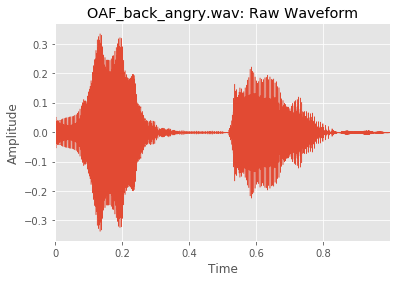
\includegraphics[width=2.7in]{figures/waveform_no.png}
    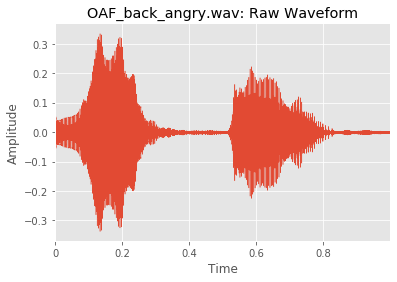
\includegraphics[width=2.7in]{figures/waveform_light.png}
    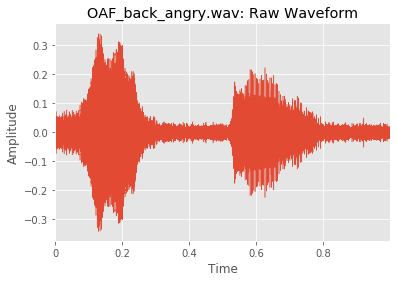
\includegraphics[width=2.7in]{figures/waveform_heavy.png}
    \captionof{figure}{Comparison of the raw waveform plots of a clean (top), light noise (middle), and heavy noise (bottom) sample. \newline}
    \label{waves}
}

The pre-processing was completed in Python using a package called Librosa \cite{youtube_2020}.
The data is prepared as a JSON file for easy importing and organization with our main models.
In addition to the raw data, two additional data sets were created from passing random Gaussian noise over each audio file.
For the light noise, the variance is only 0.001, and for the heavy noise the variance is 0.01.
These three varying levels of noise will be used to analyze the robustness of our models later.
Fig. \ref{waves} shows the waveform for each type of data.

\subsection*{Implementation Details}
Since audio is a type of time series data, it is important to recognize that the MFCC feature extraction process occurs over the whole duration of the sound clip.
In order to ensure every data point is consistent, the beginning part of every sample was clipped to fix the length of every sample at one second.
Additionally, the sampling rate for the audio is at the standard of 22050 samples per second, so, each data point begins with 22050 samples exactly.

Moreover, the standard hop-length of 512 samples is used.
The hop-length is useful for considering smaller vignettes from each full audio file; it is the number of samples we ``slide" over between one calculation of MFCC features.
So, since the sampling rate
This process results in a 13 (features) x 44 (time) matrix of MFCC features as the final product.
Fig. \ref{mfcc} is a visualization of one sample with no noise added.

{
    \centering
    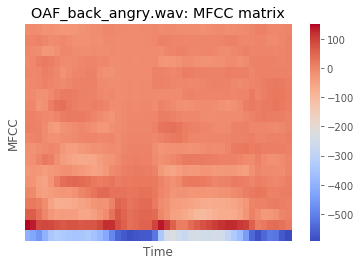
\includegraphics[width=2.75in]{figures/mfcc.png}
    \captionof{figure}{MFCC feature matrix; the visualization of the pre-processed data. \newline}
    \label{mfcc}
}

\section*{Support Vector Classifier}
Support Vector Machine (SVM) is a non-linear supervised classification algorithm which maps data into a feature space of high dimension and then uses an optimal hyperplane to separate different categories based on the maximum external separation and minimum internal difference principle \cite{suykens1999least}.

\subsection*{Implementation Details}
SVM has kernel functions such as radial basis function (RBF), polynomials, and splines that can be employed in the supervising environment. SVM has another parameter C which is the penalty of misclassification; large C brings low bias and high variance and small C brings high bias and low variance. In addition, Gamma is another parameter which is used to handle non-linear classification. A small gamma will give you high variance and low bias, meanwhile a large gamma will give you low variance and higher bias \cite{min2005bankruptcy}. In this case, comparing the accuracy of different kernel functions and parameters via grid search, we find that RBF as the kernel function, C = 50, and gamma = 1 has the best classification performance.

MFCC Feature values are extracted from raw speech signals with their class labels as mentioned earlier. We randomly shuffle the samples and employ 5-fold cross-validation in all samples to calculate the average testing accuracy. This cross-validation approach allows us to test all samples and avoids overlapping test data.

\subsection*{Results}
We utilized all three speech signals with light noisy and heave noisy to verify the overall robustness of the MFCC-SVM model. The micro-average ROC curve for each data sample is shown in Fig.\ref{figure:mfcc}.

From Fig.\ref{figure:mfcc}, we can find the area under the ROC curve of the model for the no noise speech samples is 0.99, from light noise speech samples is 0.99, and from the heavy noisy speech samples is 0.98. The MFCC-SVM model has good performance for emotional recognition. Also, it has a very strong anti-interference ability; even the wave data with heavy noise has a high AUC value in recognition. 

To further verify MFCC-SVM is a good and robust model, we employed the result obtained from another SVM model using data pre-processed with the wavelet function as a comparison \cite{zhang2004wavelet}. The time and frequency features extracted from the wavelet function are trained with an identical SVM approach. The ROC curve of the Wavelet Function-SVM (WF-SVM) is shown in Fig. \ref{figure:wf}. In this model, the AUC value from the no noise speech samples is 0.93, from light noise speech samples is 0.91, and from the heavy noise speech samples is 0.8. The performance in the WF-SVM model is not nearly as good, and the anti-interference ability of the model is poor because the result from heavy speech decreased a significant amount.

We repeated the MFCC-SVM and WF-SVM 20 times. The results of the accuracy scores of both the MFCC-SVM model and the WF-SVM model are shown in Fig.\ref{accuracy} and Tab.\ref{table:accuracy}. The accuracy scores of classification from the MFCC-SVM model by using the clean and light noise data sets are in the range of 0.94 to 0.96. Additionally, the accuracy scores for the heavy noise data are in the range of 0.88 to 0.9. The accuracy scores of classification from WF-SVM model by using clean and light noise data are in the range of 0.78 to 0.83, and the accuracy scores of the heavy noise data are in the range of 0.67 to 0.71. We can find that the accuracy scores from the MFCC-SVM model is much greater, and with far less variance than is from the WF-SVM model. Hence, the pre-processed data with MFCC has better performance than that with the Wavelet Function in terms of accuracy, stability, and anti-interference ability.

{
    \centering
    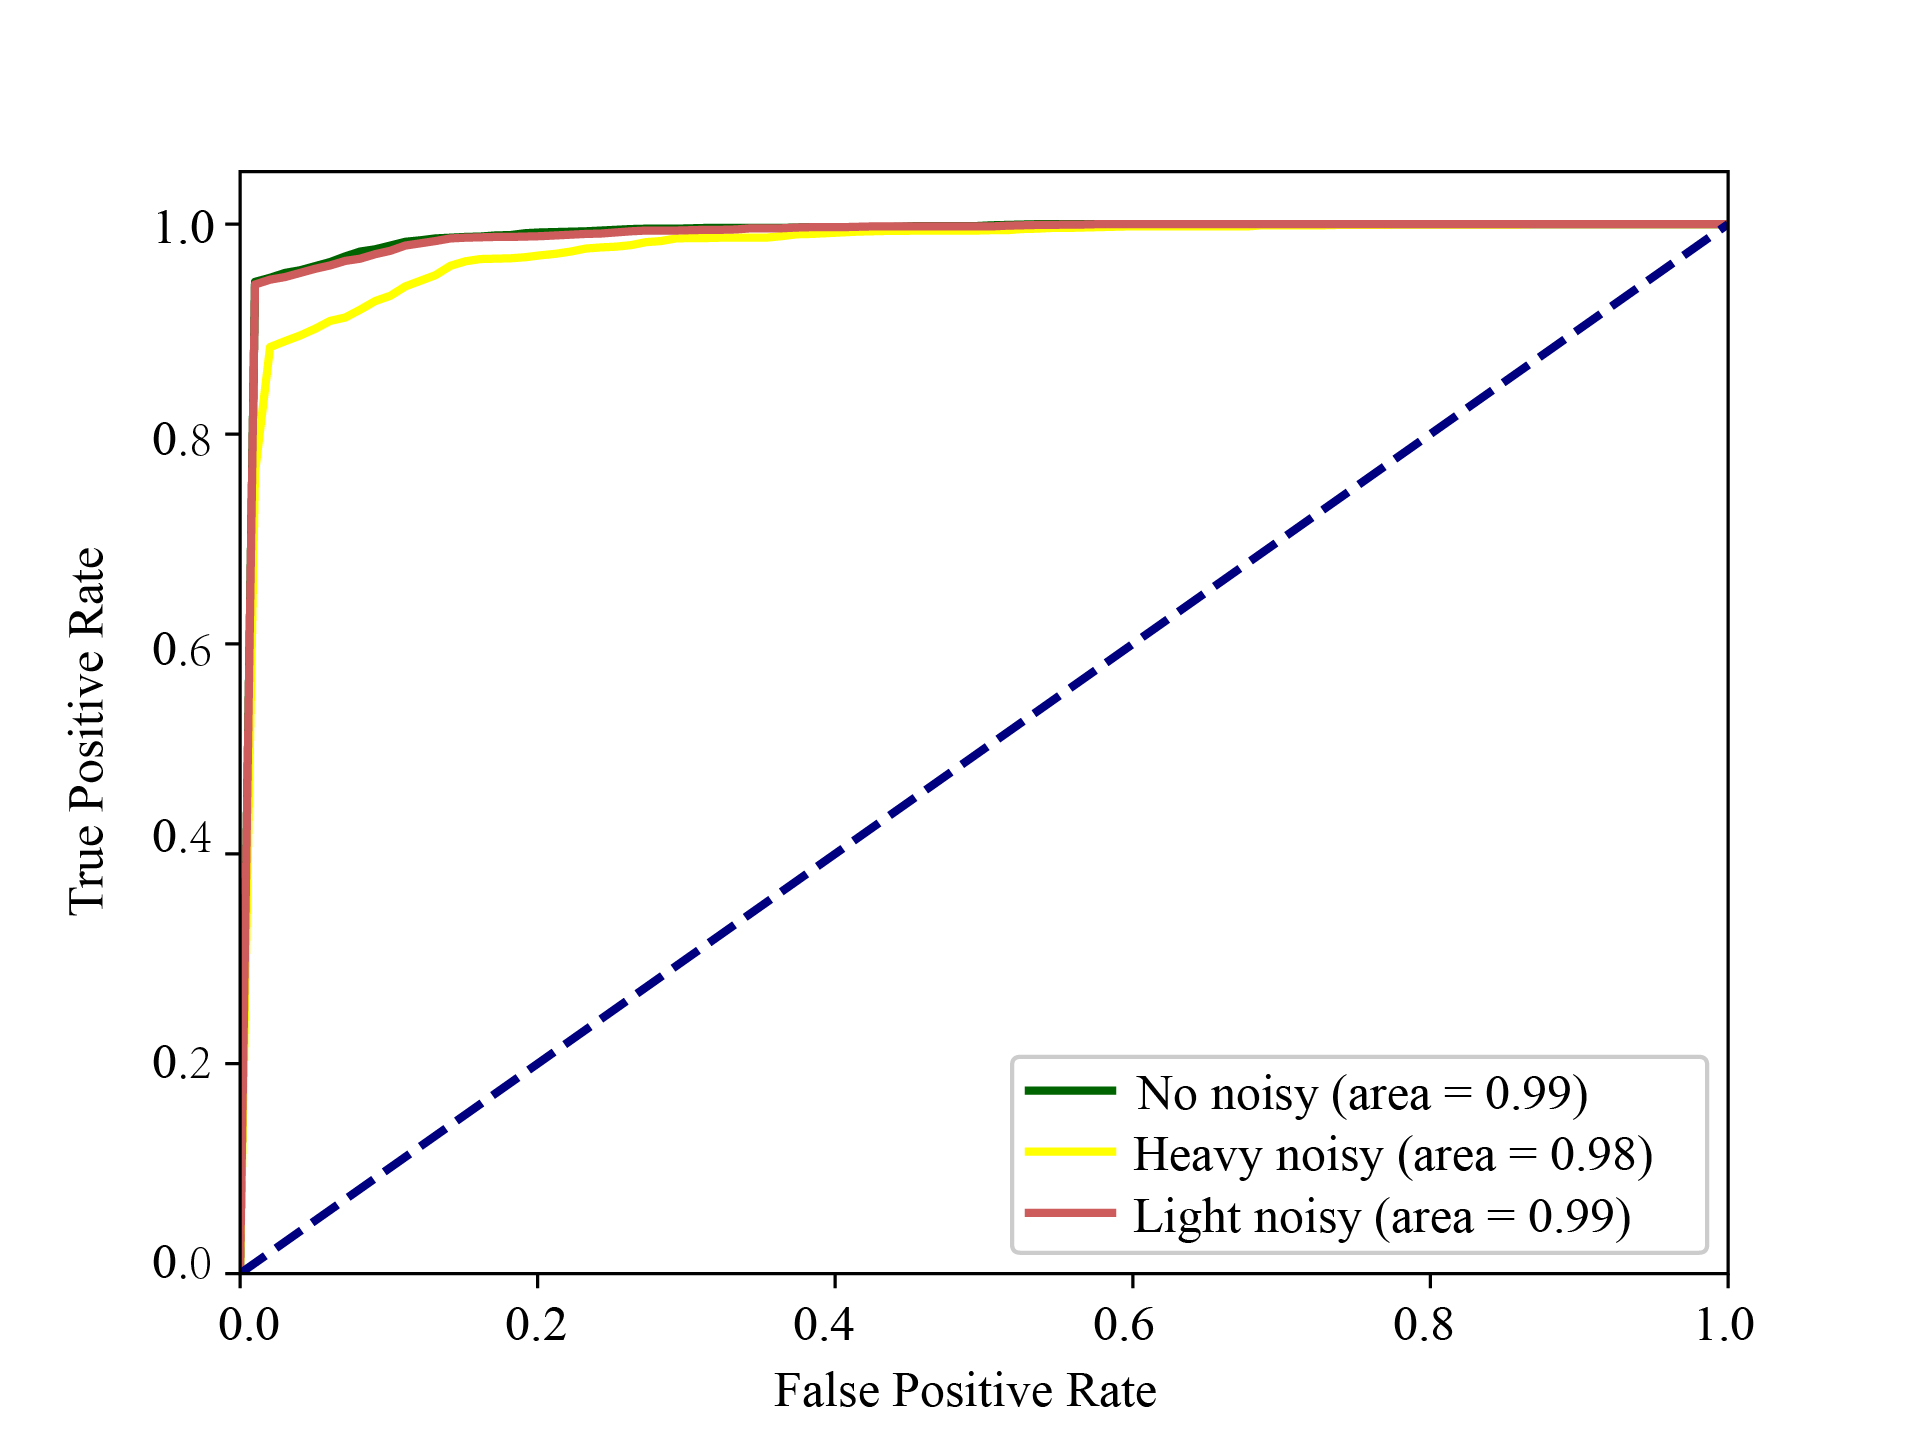
\includegraphics[width=3in]{figures/MFCC_7labels.jpg}
    \captionof{figure}{ROC of multi-class from MFCC. \newline}
    \label{figure:mfcc}
}

{
    \centering
    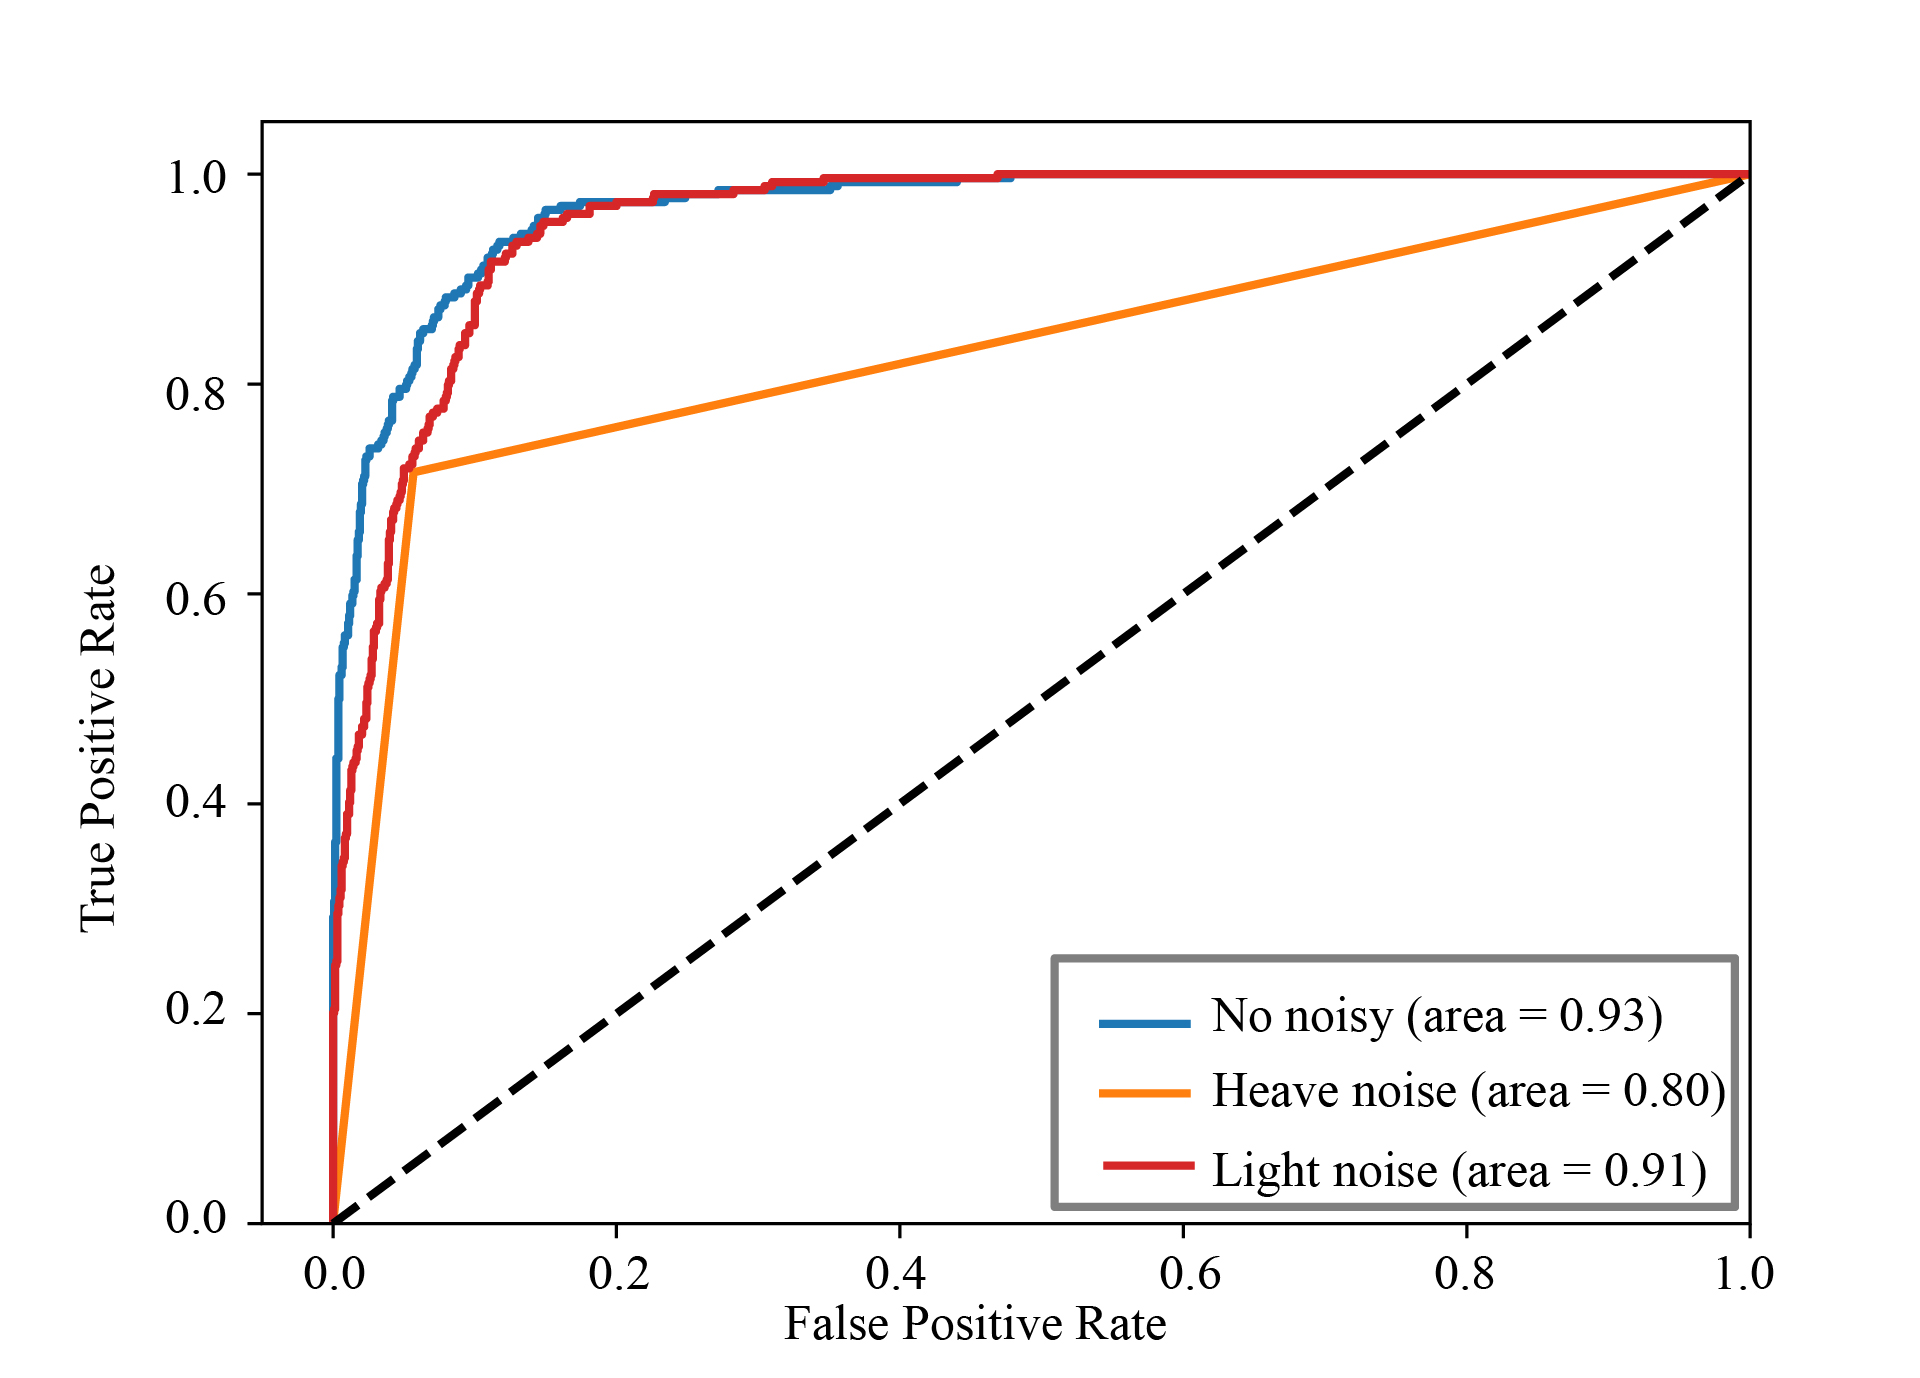
\includegraphics[width=3in]{figures/WF_7labels.jpg}
    \captionof{figure}{ROC of multi-class from Wavelet Function.}
    \label{figure:wf}
}

{
    \centering
    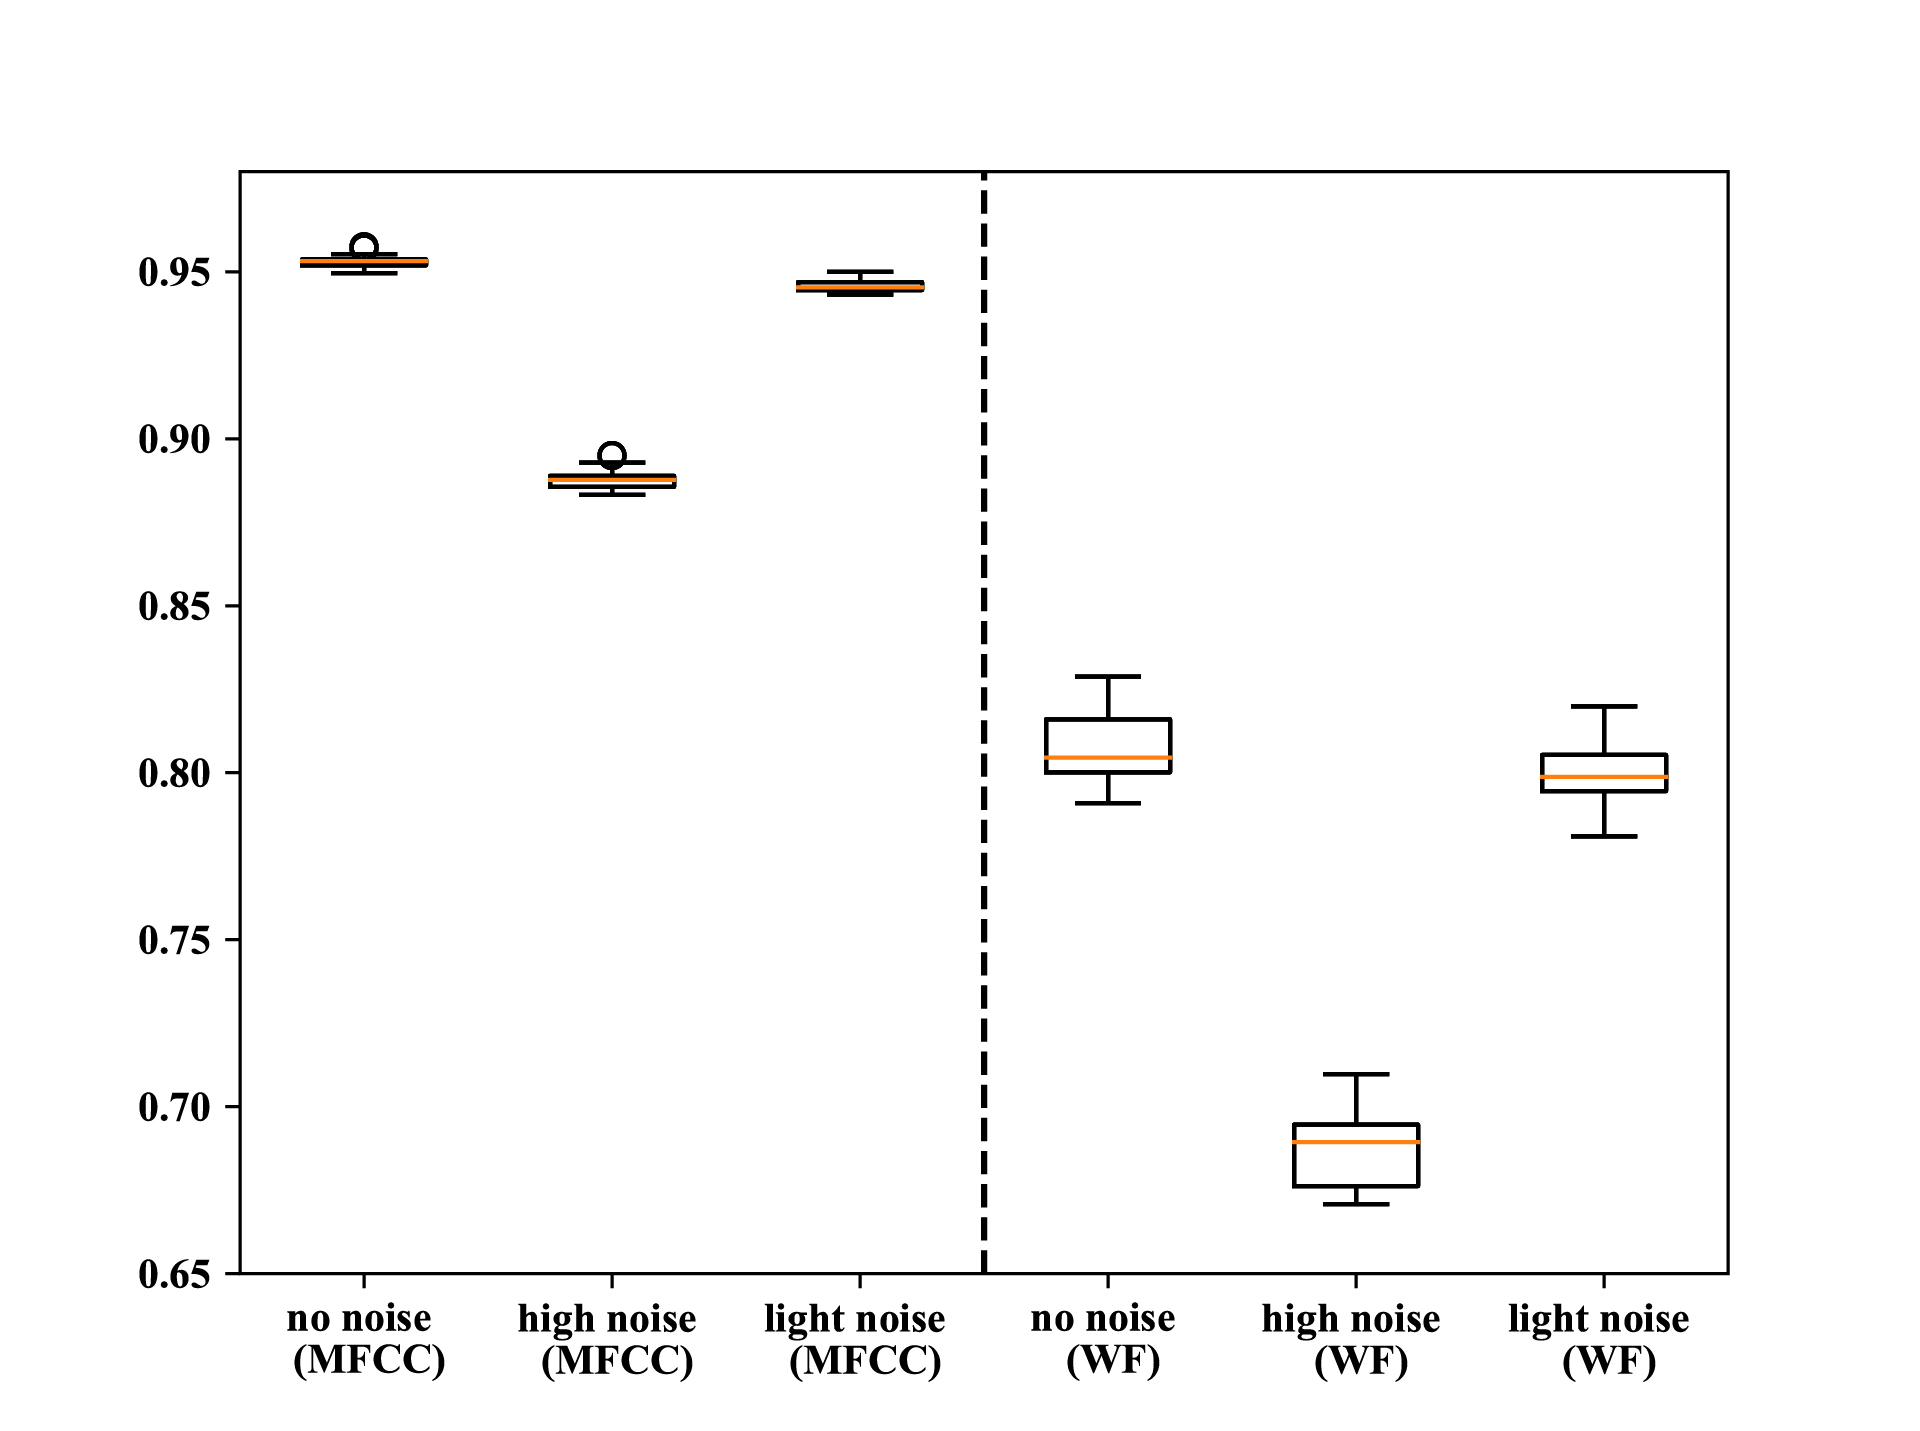
\includegraphics[width=3in]{figures/Accuracy.jpg}
    \captionof{figure}{The accuracy of classification from MFCC and Wavelet Function}
    \label{accuracy}
}

\begin{table*}[htbp]
\centering
\caption{The accuracy of classification from MFCC-SVM models and WF-SVM models}
\label{table:accuracy}
\begin{tabular}{ccccc}
\hline
\textbf{Model}                      & \textbf{Data}        & \textbf{Average} & \textbf{Standard Deviation}  & \textbf{Range}                            \\ \hline
                                    & \textbf{No noise}    & 0.953            & {\color[HTML]{000000} 0.002} & {\color[HTML]{000000} {[}0.949, 0.958{]}} \\
                                    & \textbf{Light noise} & 0.888            & {\color[HTML]{000000} 0.003} & {\color[HTML]{000000} {[}0.883, 0.895{]}} \\
\multirow{-3}{*}{\textbf{MFCC-SVM}} & \textbf{Heavy noise} & 0.946            & 0.002                        & {[}0.943, 0.950{]}                        \\
                                    & \textbf{No noise}    & 0.808            & 0.012                        & {[}0.791, 0.829{]}                        \\
                                    & \textbf{Light noise} & 0.689            & 0.013                        & {[}0.671, 00.710{]}                       \\
\multirow{-3}{*}{\textbf{WF-SVM}}   & \textbf{Heavy noise} & 0.799            & 0.012                        & {[}0.781, 0.820{]} \\
\hline
\end{tabular}
\end{table*}

\section*{Deep Learning Approach}
To better compare the classification performance of our SVM we wanted to compare the results to that of an alternative framework. We decided to employ deep learning methods because they are currently a leading industry standard for sound and image classification \cite{Nielsen2019}. 
Deep learning as a method is simply an extension of basic single layer neural networks, known also as "shallow" neural networks. Opposing these shallow networks, any neural network with two or more hidden layers is classified as deep learning \cite{Nielsen2019}. Within this broad category many architectures for networks exist, some better for specific purposes then others. 

\subsection*{Implementation Details}
For the work here, two architectures were chosen. The first is a classic deep multi-layer perceptron (MLP). While one of the earliest constructed architectures, it can be a reliable choice for the right task with the right activation function and learning rate. In addition to this, we used one of the more cutting edge approaches known as a convolutional networks. To assist with building the networks we used the python library TensorFlow \cite{youtube_2020}. This library essentially allows you to build various neural net architectures using a set of predefined functions as building blocks. For data, only the MFCC prepossessed data was used on the neural networks because this data had performed better with the SVM and we desired a direct comparison.

{
    \centering
    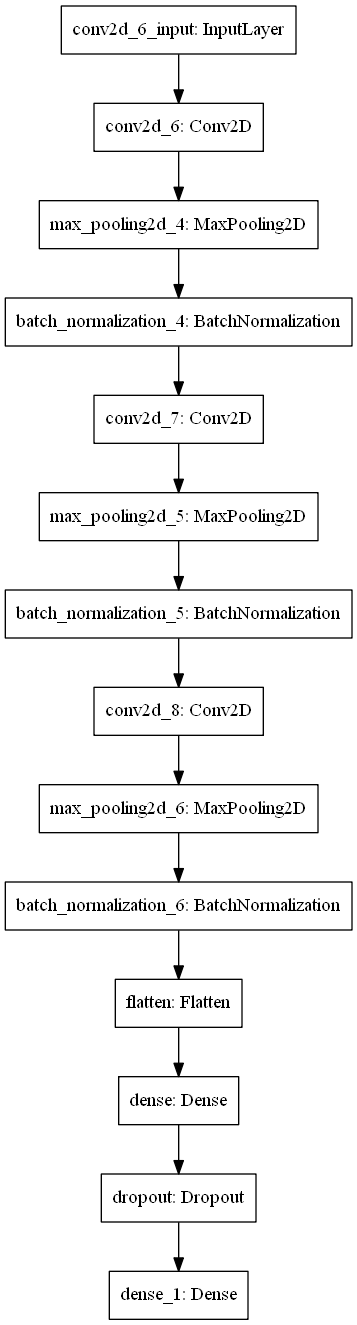
\includegraphics[width=1.74in]{figures/multi_input_and_output_model.png}
    \captionof{figure}{CNN architecture diagram. \newline}
    \label{cnn_architecture}
}

The MLP consisted of 3 hidden layers along with an input and output layer. A fourth layer was added during testing, but it gave worse results so it was removed. A learning rate of 0.0001 was used after trying 0.01 and 0.001. For learning, 100 epochs and a batch size of 20 were used after trying several different options.The hidden layers all use the ReLU activation function. It was found that the sigmoid activation function gave worse results.

For the convolutional network, three convolutional layers consisting of several functions were used. Much like the MLP, the ReLU activation function was used for its better performance. A learning rate of 0.0001 was also used. For training a batch size of 30 was used and the model ran for 50 epochs. It was then evaluated on a separate test set consisting of data not used during training. A diagram of the conceptual network structure can be seen in Fig. \ref{cnn_architecture}. 

\subsection*{Results}
The MLP was trained several times to test different learning parameters. All of the runs had training accuracy of over 0.9 and test accuracy of at least 0.83 on the clean data set. The greatest accuracy on the clean test set reached by this model was 0.9, illustrated in Fig. \ref{mlp_accuracy}. We see that this model has much room for improvement and is not the best choice already, and this is before we even consider the noise.

When the trained model was applied to the two data sets with noise, the accuracy quickly deteriorated. In the last run, the accuracy on the light noise data set was .71 and on the heavy noise data set it was .42, showing that unfortunately this network is not robust to variation in the data at all. 

A similar pattern of results was seen in the convolutional network approach. On the initial clean data set, the CNN exceeded the accuracy of the MLP by the final run with a score of 0.96 on the test set. With more time spent on optimization, this result most likely could of been improved. The training and test accuracy is captured in Fig. \ref{cnn_accuracy}.

Despite the high accuracy during training, the CNN network suffered from the same shortfalls as the MLP when new data was introduced via adding noise. Both the light and heavy noise added to original data destroyed the accuracy of the CNN, showing the superiority in the robustness of the SVM method. The light noise addition brought the accuracy down to 0.629 while the heavy noise result seemed hopeless; it was consistently around 0.15 showing this was worse than guessing the class randomly.

{
    \centering
    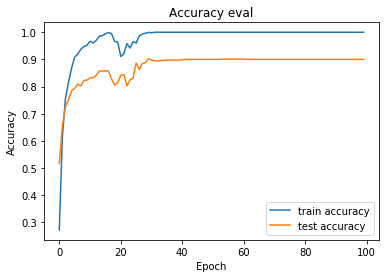
\includegraphics[width=3in]{figures/mlp_accuracy_plot2.png}
    \captionof{figure}{The accuracy of classification from MLP architecture. \newline}
    \label{mlp_accuracy}
}

{
    \centering
    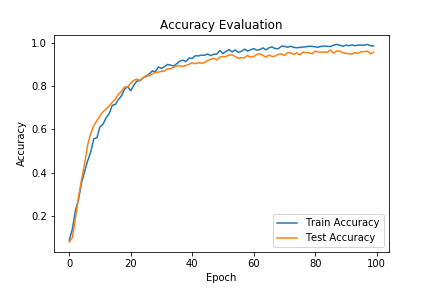
\includegraphics[width=\linewidth]{figures/cnn_initial_accuracy.png}
    \captionof{figure}{CNN architecture accuracy. \newline}
    \label{cnn_accuracy}
}

\section*{Conclusions}
To recap, we first reinforced that MFCC should be the preferred method for audio pre-processing. MFCC Features are the most accurate and robust method for extracting features for training machine learning algorithms. Our experiment shows that MFCC significantly outperforms the Wavelet Function, and other literature we have reviewed comparing other pre-processing methods all conclude with MFCC outperforming other methods.

Second, we verified that the MFCC-SVM is very robust against added Gaussian noise. When heavy and light amounts of noise were passed over the waveform data, the MFCC-SVM saw little to no degradation of performance. Hence, we conclude that the MFCC-SVM is robust against this type of noise.

Third, we explored the effects of Gaussian noise on deep learning architectures and found that they are drastically effected by this addition. Hence, we conclude that deep learning is not robust against adding noise to the system. It was the case that the deep MLP actually performed better than the CNN when noise was introduced, even though CNNs are universally a higher performing architecture. One theoretical explanation from intuition comes from looking at the log-spectrogram's of the sound samples, which can be seen in Fig. \ref{spec}.


While the effects of the noise are not very visible from the MFCC matrix, from the log-spectrogram we can see better how the noise is removing features from the spectrogram matrix. Intuitively, we know that CNNs extract features from their input data before passing those features into the deep learning architecture. Since the noise has destroyed many of those features, it is harder for the CNN to extract features from the MFCC matrix, hence causing it to perform much worse than even just the MLP. Alternatively, a traditional machine learning algorithm like an SVM relies on statistical methodology, which is more precise and less reliant on ``black box" mathematics.

{
    \centering
    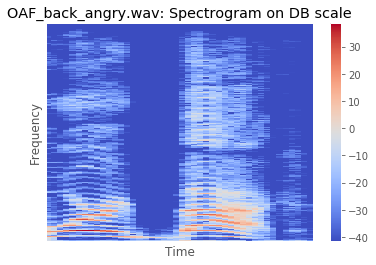
\includegraphics[width=3in]{figures/spec-no.png}
    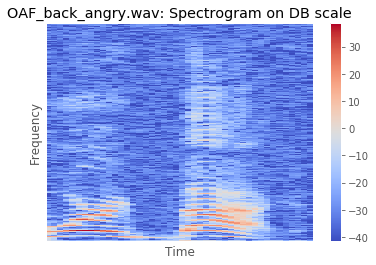
\includegraphics[width=3in]{figures/spec-light.png}
    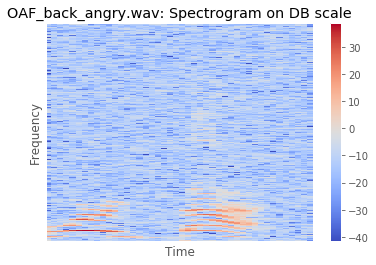
\includegraphics[width=3in]{figures/spec-heavy.png}
    \captionof{figure}{Comparison of the log-spectrogram between a no noise sample (top), light noise (middle), and heavy noise (bottom).\newline}
    \label{spec}
}

\section*{Limitations; Future Work}
The largest and most glaring limitation to this work is the data being used. The TESS data set is very good, but suffers from the lack of variety in subjects. We call this problem the ``Heterogeneous Data'' problem, and it is prevalent with human subjects. Heterogeneous data is very high in variability and can be ambiguous due to having a poor representation in a data set \cite{wang2017heterogeneous}. For example, in the TESS data set, there are no male voices present. If we were to test the emotion classification using a male voice it is likely to not do as well because there can be significant differences in pitch and tone from a male voice than from one of the actors from the TESS data.

There are two ways to combat these limitations in future works. The first way is to use a data set that captures more variability. However this can be much easier said than done. assembling thousands of participants to collect voice recordings is a large task in and of itself. Moreover, a few thousand participants still is not enough to represent a population for something as unique and variable as the human voice. Not to mention, there are hundreds of languages, all with different nuance that introduces even \emph{more} variability in this system. Albeit, having a data set, even with a few dozen different participants would be a large improvement to begin with.

The second proposed solution to this problem is much more realistic and immediate for future work. More variability can be artificially introduced into the system via computational tools. For example, in addition to adding noise to the system, other components can be changed such as pitch, or pacing. This can be done randomly as well to roughly simulate more heterogeneity in the data.

\appendix
\section{Source Code}
The source code for this project is available on GitHub with the following link:
\begin{center}
\bf{https://github.com/cwolosh1/emotion-classification}
\end{center}

\bibliographystyle{IEEEtran}
\bibliography{citations}
\end{multicols*}
\end{document}